\documentclass[times, utf8, seminar, numeric]{fer}

\usepackage{booktabs}
\usepackage{hyperref}
\usepackage{enumitem}
\usepackage{mathtools}
\usepackage{listings}
\usepackage{tikz-uml}
\usepackage[croatian, algoruled, noend, lined, linesnumbered, algochapter]{algorithm2e}
\usepackage{multirow}
\usepackage{tikz}
\usepackage{svg}

\begin{document}

\title{Sybil napadi u društvenim mrežama i zaštita od njih}
\author{Antun Razum}
\voditelj{prof. dr. sc. Siniša Srbljić}

\maketitle

\tableofcontents

\chapter{Uvod}
\textit{Sybil} napadi \engl{Sybil attacks} su dobro poznata vrsta napada u distribuiranim sustavima poput senzorskih i \textit{peer-to-peer} mreža. U osnovnom obliku ovog napada napadač stori velik broj lažnih identiteta preko kojih utječe na ponašanje napadnutog sustava. Broj identiteta koji napadač može stvoriti ovisi o napadačevim resursima kao što su propusnost mreže, memorija i računarna moć.

%TODO: Napiši poglavlje

\chapter{Sybil napadi}
\begin{figure}[h]
	\centering
	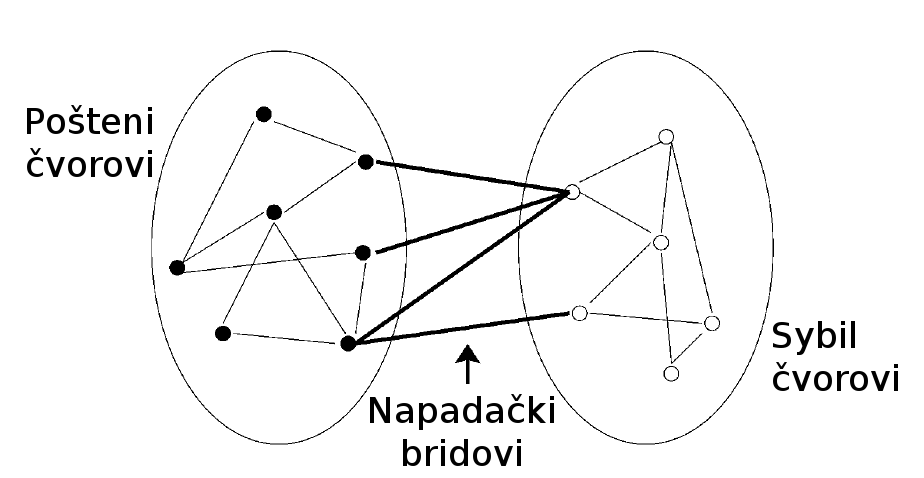
\includegraphics[scale=0.3]{attack.png}
	\caption{Napadački bridovi u grafu društvene mreže}
	\label{fig:attack}
\end{figure}

%TODO: uvod u poglavlje

\section{Povijest i motivacija}
%TODO: uvod u odjeljak

\subsection{Središnji autoritet}
Sybil napadi mogu se lagano kontrolirati pomoću pouzdranog središnjeg autoriteta koji izdaje i provjerava podatke jedinstvene stvarnom čovjeku. Na primjer, ako sustav zahtijeva registraciju korisnika pomoću broja osobne iskaznice ili vozačke dozvole, onda prepreka za sybil napade postaje puno viša. Autoritet također može zahtijevati i plaćanje za registraciju. Nažalost, postoje mnogi slučajevi gdje takvi sustavi nisu poželjni. Na primjer, može biti teško izabrati jedinstveni autoritet kome mogu vjerovati svi korisnici na svijetu. Nadalje, taj središnji autoritet može lako postati točka zatajenja \engl{single point of failure} -- meta \textit{denial-of-service} napada ili usko grlo u izvođenju sustava. Na poslijetku, plaćanje registracije ili traženje osjetljivih informacija prilikom iste odbilo bi velik broj korisnika. Jedini način da se ovi problemi izbjegnu je distribuiranost sustava za provjeru. \cite{sybil-guard}

\subsection{Izazovi u decentraliziranim pristupima}
Obrana od sybil napada bez puzdanog središnjeg autoriteta puno je teža. Puno decentraliziranih sustava pokušavalo se boriti protiv sybil napada povezivanjem identiteta korisnika s IP adresom. No, napadačima još tada korištenjem određenih metoda nije bio problem ukrasti i iskoristiti veći broj IP adresa s kojih mogu djelovati. \cite{spammers} Osim krađe IP adresa, napadač može preuzeti veći broj korisničkih računala tako stvarajući \textit{botnet} sačinjen od tisuća računala diljem svijeta. Mnogi drugi decentralizirani načini obrane također su se pokazali neuspješnima. Primjerice zagonetke koje zahtijevaju ljudski napor, kao što je \textit{CAPTCHA}, napadač može upotrijebiti na svojoj stranici tražeći od korisnika njegove stranice da ih riješe. Sve to vodi do zaključka kako se obrana od napada ne može temeljiti na jednokratnim provjerama prilikom registracije korisnika na sustav, već na temeljitoj analizi grafa društvene mreže te ispitivanju na raznih algoritamskih svojstava grafa. \cite{sybil-guard}

\section{Pojmovi i definicije}
%TODO: uvod u odjeljak

\subsection{Model sustava}
Društvena mreža promatra se kao neusmjereni beztežinski graf $G = (V, E)$. Čvorovi predstavljaju korisnike mreže, a bridovi određenu vrstu odnosa između korisnika. Vrijedi $|V| = n, V = {v_1, v_2, ..., v_n}$ te $|E| = m$, gdje je $e_{ij} \in E$ tj. $v_i \to v_j$ ako je $v_i \in V$ susjedan $v_j \in V$, za $1 \leq i, j \leq n$. Matrica $A = [a_{ij}]^{n \times n}$ naziva se matrica susjedstva gdje je $a_{ij} = 1$ ako je $e_{ij} \in E$ i $a_{ij} = 0$ ako nije. Matrica $P = [p_{ij}]^{n \times n}$ naziva se matrica prijelaza \engl{transition matrix}
\begin{equation} \label{eq:transition}
  p_{ij} = 
  \begin{cases}
    \frac{1}{deg(v_i)} & e_{ij} \in E \\
    0 & inace \\
  \end{cases}
\end{equation}
gdje je $deg(v_i)$ stupanj čvora $v_i$. Skup susjeda čvora $v_i$ označava se s $N(v_i)$ tako da je $deg(v_i) = |N(v_i)|$.

U mreži se nalazi određeni broj \textit{poštenih čvorova} \engl{honest nodes}, svaki sa svojim identitetom, koji predstavljaju stvarne korisnike mreže. Također postoji jedan ili više napadača u mreži, svaki s određenim brojem lažnih identiteta koji su u grafu predstavljeni \textit{sybil čvorovima}. Bridovi između sybil čvorova i poštenih čvorova nazivaju se \textit{napadački bridovi} \engl{attack edges}. \textit{Sybil regija} \engl{sybil region} sastoji se od svih sybil čvorova, a \textit{poštena regija} \engl{honest region} sastoji se od svih poštenih čvorova. Sve sybil čvorove kontrolira napadač. Stoga, napadač može stvoriti proizvoljan broj bridova unutar sybil regije.

\subsection{Slučajne šetnje i vrijeme miješanja}
Prijelaz između dva čvora u grafu može se prikazati markovljevim lancem (ML) koji predstavlja slučajnu štetnju kroz graf $G$. \textit{Slučajna šetnja} duljine $w$ preko $G$ je niz čvorova u $G$ koji počinje čvorom $v_i$ i završava čvorom $v_t$. ML je ergodičan \engl{ergodic} ako je ireducibilan i aperiodičan, što znači da ima stacionarnu distribuciju $\pi$ i distribucija poslije slučajne šetnje duljine $w$ konvergira prema $\pi$ kada $w \to \infty$. Stacionarna distribucija ML je distribucija koja je invarijantna s obrizorm na matricu prijelaza $P$ tj. $\pi P = \pi$. \textit{Vrijeme miješanja} \engl{mixing time} ML definira se kao najmanja duljina slučajne šetnje kojom se postiže stacionarna distribucija. Formalno i preciznije, ovu definiciju možemo izreći na sljedeći način:
\begin{equation} \label{eq:mixing}
  T(\epsilon) = \max_{i} \min \{t : |\pi - \pi^{(i)} P^t|_1 < \epsilon\}
\end{equation}
gdje je $\pi$ stacionarna distribucija, $\pi^{(i)}$ početna distribucija koncentrirana na čvoru $v_i$, $P^t$ matrica prijelaza nakon $t$ koraka, a $|\cdot|_1$ ukupna varijacijska udaljenost, definirana kao $\frac{1}{2} \sum_{j} |\pi_j - \pi_j^{(i)}|$. Za ML kažemo da je \textit{brzo miješajući} \engl{rapidly mixing, fast mixing} ako je $T(\epsilon) = O(\log n)$. \cite{friends} 

\textit{Teorem o stacionarnoj distribuciji}: Za neusmjereni beztežinski graf $G$, stacionarna distribucija ML preko $G$ je vektor $\pi = [\pi_{v_i}]$ gdje je $\pi_{v_i} = \frac{deg (v_i)}{2 m}$ tj. $\pi = [\frac{deg (v_1)}{2 m} \frac{deg (v_2)}{2 m} \dots \frac{deg (v_n)}{2 m}]$.

Uz pomoć prethodnog teorema može se dokazati da je vrijeme miješanja u korelaciji s povezanošću grafa. Dobro povezani grafovi imaju malo vrijeme miješanja, dok slabo povezani grafovi imaju veće vrijeme miješanja. \cite{friends}

\chapter{Obrana od sybil napada}

\section{Pretpostavke}
Algoritmi za obranu od sybil napda temelje se na sljedećim pretpostavkama za koje se pokazalo da vrijede u stvarnim društvenim mrežama \cite{sybil-defender}:

\textbf{Poštena regija je brzo miješajuća.} Kao što je definirano u prethodnom poglavlju, to znači da vrijedi $T(\epsilon) = O(\log n)$, za funkciju vremena miješanja definiranu prema jednadžbi \ref{eq:mixing}. Slučajne šetnje u brzo miješajućim grafovima općenito brzo konvergiraju ka stacionarnoj distribuciji. \cite{sybil-defender} Pokazano je da su stvarne društvene mreže brzo miješajuće. \cite{sybil-limit}

\textbf{Jedan poznat pošteni čvor.} U grafu postoji barem jedan poznati pošteni čvor. Iz tog čvora kreće potraga za sybil čvorovima.

\textbf{Administratoru je poznata topologija društvene mreže.} Ovo povlači tvrdnju da je algoritam centraliziran. Budući da su sve današnje društvene mreže pod centraliziranom kontrolom, može se pretpostaviti da su administratori tih mreža ti koji brinu za sigurnost sustava pa tako i obranu od sybil napada.

\textbf{Veličina sybil regije nije usporediva s veličinom poštene regije.} Uz današnje veličine društvenih mreža (npr. Facebook preko 1,6 milijardi), može se pretpostaviti da je napadaču nemoguće stvoriti toliko sybil identiteta. To je tim više otežano uobičajenim postupcima provjere korisnika kao što su potvrda e-mail adrese, unos osobnih informacija te rješavanje CAPTCHA-e.

\textbf{Broj napadačkih bridova je ograničen.} Kao posljedica, kada napadač stvori veći broj sybil čvorova, postojat će nepropocijonalno mali \textit{rez} (rezni skup) između poštene i sybil regije. Postojanje malog reza narušava svojstvo brzog miješanja: miješanje između poštenih čvorova je brzo, dok je miješanje između poštenih i sybil čvorova sporo.

\section{Algoritam}
Cjelokupni algoritam sastoji se od tri komponente: algoritma za identifikaciju sybil čvorova, algoritma za detekciju sybil grupa te dva pristupa ograničavanju broja napadačkih bridova. Tri se komponente mogu koristiti u konjunkciji za što bolju obranu. \cite{sybil-defender}
%TODO: Uvod u odjeljak

\subsection{Algoritam za identifikaciju sybil čvorova}
Algoritam za identifikaciju sybil čvorova prima graf društvene mreže $G(V, E)$, poznati pošteni čvor $h$ i \textit{osumnjičeni čvor} \engl{suspect node} $u$ kao ulaz, a vraća je li čvor $u$ uistinu syibil čvor ili ne. Algoritam se temelji na slučajnim šetnjama. Slučajna šetnja na grafu definirana je nizom prijelaza između čvorova grafa $G$. Ako je šetnja u nekom koraku na čvoru $v_i$, onda je vjerojatnost da će se šetnja nastaviti preko brida $v_i \to v_j$ jednaka $\frac{1}{deg(v_i)}$ prema jednadžbi \ref{eq:transition}.

Intuicija algoritma je sljedeća: budući da je rez između poštene i sybil regije mali, slučajne šetnje koje polaze od sybil čvorova u pravilu će zapeti u sybil regiji. Također, zbog pretpostavke o neusporedivosti veličine sybil regije i poštene regije, broj čvorova prijeđenih slučajnm šetnjama iz poštenih čvorova bit će veći od broja čvorova prijeđenih šetnjama iz sybil čvorova sve dok su šetnje dovoljno dugačke i dok je broj šetnji dovoljno velik da se ta razlika istakne. Poradi daljnjih objašnjenja, broj prijelaza skupa slučajnih šetnji preko određenog čvora definira se kao \textit{frekvencija} tog čvora. Valja primijetiti da neki čvor može biti prijeđen više puta u jednoj šetnji.

Algoritam za identifikaciju sybil čvorova sastoji se od dvije faze opisane u algoritmima \ref{alg:identify1} i \ref{alg:identify2}. Prva faza prima graf $G$ i $h$ kao ulaze i vraća pragove koje koristi druga faza kako bi identificirala sybil čvorove. Prva se faza treba pozvati samo jednom za cijeli graf društvene mreže. Kao što je pokazano u algoritmu \ref{alg:identify1}, algoritam prvo napravi $f$ kratkih slučajnih štetnji duljine $l_s = \log n$ iz poznatog poštenog čvora $h$.

\begin{algorithm}[h]
	\caption{Računanje pragova}
	\label{alg:identify1}
\end{algorithm}

\begin{algorithm}[h]
	\caption{Identifikacija sybil čvorova}
	\label{alg:identify2}
\end{algorithm}

\chapter{Zaključak}
%TODO: Napiši poglavlje

\bibliography{literatura}
\bibliographystyle{fer}

\begin{sazetak}
  Sybil napad je napad kojim se pokušava srušiti sustav reputacije stvaranjem lažnih identiteta u peer-to-peer mrežama koji djeluju na slican način. Društvene mreže su vrlo česta meta sybil napada. Zaštita od sybil napada na društevnim mrežama temelji se na algoritamskim svojstvima grafova društevnih mreža putem kojih se računa razina povjerenja koja se može pridijeliti proizvoljnom čvoru grafa.

  \kljucnerijeci{društvene mreže, sybil napad, teorija grafova, sigurnost podataka, idenditet}
\end{sazetak}

\end{document}
